% ******************************* PhD Thesis Template **************************
% Please have a look at the README.md file for info on how to use the template

\documentclass[a4paper,12pt,customfont,custombib,draft,index,custommargin,oneside]{Classes/PhDThesisPSnPDF}

% ******************************************************************************
% ******************************* Class Options ********************************
% *********************** See README for more details **************************
% ******************************************************************************

% `a4paper'(The University of Cambridge PhD thesis guidelines recommends a page
% size a4 - default option) or `a5paper': A5 Paper size is also allowed as per
% the Cambridge University Engineering Deparment guidelines for PhD thesis
%
% `11pt' or `12pt'(default): Font Size 10pt is NOT recommended by the University
% guidelines
%
% `oneside' or `twoside'(default): Printing double side (twoside) or single
% side.
%
% `print': Use `print' for print version with appropriate margins and page
% layout. Leaving the options field blank will activate Online version.
%
% `index': For index at the end of the thesis
%
% `draftclassic': For draft mode without loading any images (same as draft in book)
%
% `draft': Special draft mode with line numbers, images, and water mark with
% timestamp and custom text. Position of the text can also be modified.
%
% `abstract': To generate only the title page and abstract page with
% dissertation title and name, to submit to the Student Registry
%
% `chapter`: This option enables only the specified chapter and it's references
%  Useful for review and corrections.
%
% ************************* Custom Page Margins ********************************
%
% `custommargin`: Use `custommargin' in options to activate custom page margins,
% which can be defined in the preamble.tex. Custom margin will override
% print/online margin setup.
%
% *********************** Choosing the Fonts in Class Options ******************
%
% `times' : Times font with math support. (The Cambridge University guidelines
% recommend using times)
%
% `fourier': Utopia Font with Fourier Math font (Font has to be installed)
%            It's a free font.
%
% `customfont': Use `customfont' option in the document class and load the
% package in the preamble.tex
%
% default or leave empty: `Latin Modern' font will be loaded.
%
% ********************** Choosing the Bibliography style ***********************
%
% `authoryear': For author-year citation eg., Krishna (2013)
%
% `numbered': (Default Option) For numbered and sorted citation e.g., [1,5,2]
%
% `custombib': Define your own bibliography style in the `preamble.tex' file.
%              `\RequirePackage[square, sort, numbers, authoryear]{natbib}'.
%              This can be also used to load biblatex instead of natbib
%              (See Preamble)
%
% **************************** Choosing the Page Style *************************
%
% `default (leave empty)': For Page Numbers in Header (Left Even, Right Odd) and
% Chapter Name in Header (Right Even) and Section Name (Left Odd). Blank Footer.
%
% `PageStyleI': Chapter Name next & Page Number on Even Side (Left Even).
% Section Name & Page Number in Header on Odd Side (Right Odd). Footer is empty.
%
% `PageStyleII': Chapter Name on Even Side (Left Even) in Header. Section Number
% and Section Name in Header on Odd Side (Right Odd). Page numbering in footer

% Uncomment to change page style
%\pagestyle{PageStyleII}

% ********************************** Preamble **********************************
% Preamble: Contains packages and user-defined commands and settings
% ******************************************************************************
% ****************************** Custom Margin *********************************

% Add `custommargin' in the document class options to use this section
% Set {innerside margin / outerside margin / topmargin / bottom margin}  and
% other page dimensions
\newcommand\hmmax{0}
\newcommand\bmmax{0}
\ifsetCustomMargin
  \RequirePackage[left=25mm,right=25mm,top=25mm,bottom=25mm]{geometry}
  \setFancyHdr % To apply fancy header after geometry package is loaded
\fi

% Add spaces between paragraphs
%\setlength{\parskip}{0.5em}
% Ragged bottom avoids extra whitespaces between paragraphs
\raggedbottom
% To remove the excess top spacing for enumeration, list and description
%\usepackage{enumitem}
%\setlist[enumerate,itemize,description]{topsep=0em}

% *****************************************************************************
% ******************* Fonts (like different typewriter fonts etc.)*************

% Add `customfont' in the document class option to use this section

\ifsetCustomFont
  % Set your custom font here and use `customfont' in options. Leave empty to
  % load computer modern font (default LaTeX font).
  %\RequirePackage{helvet}

  % For use with XeLaTeX
  %  \setmainfont[
  %    Path              = ./libertine/opentype/,
  %    Extension         = .otf,
  %    UprightFont = LinLibertine_R,
  %    BoldFont = LinLibertine_RZ, % Linux Libertine O Regular Semibold
  %    ItalicFont = LinLibertine_RI,
  %    BoldItalicFont = LinLibertine_RZI, % Linux Libertine O Regular Semibold Italic
  %  ]
  %  {libertine}
  %  % load font from system font
  %  \newfontfamily\libertinesystemfont{Linux Libertine O}
  \usepackage[bitstream-charter]{mathdesign}
  \DeclareMathAlphabet{\altmathcal}{OMS}{cmsy}{m}{n}
\fi

% *****************************************************************************
% **************************** Custom Packages ********************************

% ************************* Algorithms and Pseudocode **************************

\usepackage{algpseudocode}
\usepackage{algorithm}


% ********************Captions and Hyperreferencing / URL **********************

% Captions: This makes captions of figures use a boldfaced small font.
%\RequirePackage[small,bf]{caption}

\RequirePackage[labelsep=space,tableposition=top]{caption}
\renewcommand{\figurename}{Fig.} %to support older versions of captions.sty


% *************************** Graphics and figures *****************************

%\usepackage{rotating}
%\usepackage{wrapfig}

% Uncomment the following two lines to force Latex to place the figure.
% Use [H] when including graphics. Note 'H' instead of 'h'
%\usepackage{float}
%\restylefloat{figure}

% Subcaption package is also available in the sty folder you can use that by
% uncommenting the following line
% This is for people stuck with older versions of texlive
%\usepackage{sty/caption/subcaption}
\usepackage{subcaption}

% ********************************** Tables ************************************
\usepackage{booktabs} % For professional looking tables
\usepackage{multirow}

%\usepackage{multicol}
%\usepackage{longtable}
%\usepackage{tabularx}


% *********************************** SI Units *********************************
\usepackage{siunitx} % use this package module for SI units


% ******************************* Line Spacing *********************************

% Choose linespacing as appropriate. Default is one-half line spacing as per the
% University guidelines

% \doublespacing
\onehalfspacing
% \singlespacing


% ************************ Formatting / Footnote *******************************

% Don't break enumeration (etc.) across pages in an ugly manner (default 10000)
%\clubpenalty=500
%\widowpenalty=500

%\usepackage[perpage]{footmisc} %Range of footnote options


% *****************************************************************************
% *************************** Bibliography  and References ********************

%\usepackage{cleveref} %Referencing without need to explicitly state fig /table

% Add `custombib' in the document class option to use this section
\ifuseCustomBib
   \RequirePackage[square, numbers]{natbib} % CustomBib

% If you would like to use biblatex for your reference management, as opposed to the default `natbibpackage` pass the option `custombib` in the document class. Comment out the previous line to make sure you don't load the natbib package. Uncomment the following lines and specify the location of references.bib file

%\RequirePackage[backend=biber, style=numeric-comp, citestyle=numeric, sorting=nty, natbib=true]{biblatex}
%\bibliography{References/references} %Location of references.bib only for biblatex

\fi

% changes the default name `Bibliography` -> `References'
\renewcommand{\bibname}{References}


% ******************************************************************************
% ************************* User Defined Commands ******************************
% ******************************************************************************

% *********** To change the name of Table of Contents / LOF and LOT ************

%\renewcommand{\contentsname}{My Table of Contents}
%\renewcommand{\listfigurename}{My List of Figures}
%\renewcommand{\listtablename}{My List of Tables}


% ********************** TOC depth and numbering depth *************************

\setcounter{secnumdepth}{2}
\setcounter{tocdepth}{2}


% ******************************* Nomenclature *********************************

% To change the name of the Nomenclature section, uncomment the following line

%\renewcommand{\nomname}{Symbols}


% ********************************* Appendix ***********************************

% The default value of both \appendixtocname and \appendixpagename is `Appendices'. These names can all be changed via:

%\renewcommand{\appendixtocname}{List of appendices}
%\renewcommand{\appendixname}{Appndx}

% *********************** Configure Draft Mode **********************************

% Uncomment to disable figures in `draft'
%\setkeys{Gin}{draft=true}  % set draft to false to enable figures in `draft'

% These options are active only during the draft mode
% Default text is "Draft"
%\SetDraftText{DRAFT}

% Default Watermark location is top. Location (top/bottom)
%\SetDraftWMPosition{bottom}

% Draft Version - default is v1.0
%\SetDraftVersion{v1.1}

% Draft Text grayscale value (should be between 0-black and 1-white)
% Default value is 0.75
%\SetDraftGrayScale{0.8}


% ******************************** Todo Notes **********************************
%% Uncomment the following lines to have todonotes.

\ifsetDraft
	\usepackage[colorinlistoftodos]{todonotes}
	\newcommand{\mynote}[1]{\todo[author=ms2314 ,size=\small,inline,color=green!40]{#1}}
\else
	\newcommand{\mynote}[1]{}
	\newcommand{\listoftodos}{}
\fi

% Example todo: \mynote{Hey! I have a note}

% my extra stuff
\usepackage[mode=buildnew]{standalone}
%\usepackage{tikz,pgfplots}
%\standaloneconfig{mode=buildnew}

\newtheorem{theorem}{Theorem}[section]
\newtheorem{corollary}{Corollary}[theorem]
\newtheorem{lemma}[theorem]{Lemma}
\newtheorem{definition}[theorem]{Definition}

\usepackage{amsmath}
\usepackage{bm}

% ************************ Thesis Information & Meta-data **********************
% Thesis title and author information, refernce file for biblatex
% ************************ Thesis Information & Meta-data **********************
%% The title of the thesis
\title{Writing your PhD thesis in \texorpdfstring{\\ \LaTeX2e}{LaTeX2e}}
%\texorpdfstring is used for PDF metadata. Usage:
%\texorpdfstring{LaTeX_Version}{PDF Version (non-latex)} eg.,
%\texorpdfstring{$sigma$}{sigma}

%% Subtitle (Optional)
\subtitle{Using the CUED template}

%% The full name of the author
\author{Krishna Kumar}

%% Department (eg. Department of Engineering, Maths, Physics)
\dept{Department of Engineering}

%% University and Crest
\university{University of Cambridge}
% Crest minimum should be 30mm.
\crest{
\includegraphics[width=0.2\textwidth]{University_Crest}}
%% Use this crest, if you are using the college crest
%% Crest long miminum should be 65mm
%\crest{
\includegraphics[width=0.45\textwidth]{University_Crest_Long}}

%% College shield [optional] 
% Crest minimum should be 30mm.
%\collegeshield{
\includegraphics[width=0.2\textwidth]{CollegeShields/Kings}}


%% Supervisor (optional)
%% for multiple supervisors, append each supervisor with the \newline command
%\supervisor{Prof. A.B. Supervisor\newline
%Prof. C.D. Supervisor}

%% Supervisor Role (optional) - Supervisor (default) or advisor
% \supervisorrole{\textbf{Supervisors: }}
%% if no title is desired:
% \supervisorrole{}

%% Supervisor line width: required to align supervisors
%\supervisorlinewidth{0.35\textwidth}

%% Advisor (optional)
%% for multiple advisors, append each advisor with the \newline command
%\advisor{Dr. A. Advisor\newline
%Dr. B. Advisor}
     
%% Advisor Role (optional) - Advisor (default) or leave empty
% \advisorrole{Advisors: }
%% if no title is required
% \advisorrole{}

%% Advisor line width: required to align supervisors
%\advisorlinewidth{0.25\textwidth}


%% You can redefine the submission text:
% Default as per the University guidelines:
% ``This dissertation is submitted for the degree of''
%\renewcommand{\submissiontext}{change the default text here if needed}

%% Full title of the Degree
\degreetitle{Doctor of Philosophy}

%% College affiliation (optional)
\college{King's College}

%% Submission date
% Default is set as {\monthname[\the\month]\space\the\year}
%\degreedate{September 2014} 

%% Meta information
\subject{LaTeX} \keywords{{LaTeX} {PhD Thesis} {Engineering} {University of
Cambridge}}


% ***************************** Abstract Separate ******************************
% To printout only the titlepage and the abstract with the PhD title and the
% author name for submission to the Student Registry, use the `abstract' option in
% the document class.

\ifdefineAbstract
 \pagestyle{empty}
 \includeonly{Declaration/declaration, Abstract/abstract}
\fi

% ***************************** Chapter Mode ***********************************
% The chapter mode allows user to only print particular chapters with references
% Title, Contents, Frontmatter are disabled by default
% Useful option to review a particular chapter or to send it to supervisior.
% To use choose `chapter' option in the document class

\ifdefineChapter
 \includeonly{Chapter3/chapter3}
\fi

% ******************************** Front Matter ********************************
\begin{document}

\frontmatter

\maketitle

%% ******************************* Thesis Dedidcation ********************************

\begin{dedication} 

I would like to dedicate this thesis to my loving parents \dots

\end{dedication}
%% ******************************* Thesis Declaration ***************************

\begin{declaration}

I hereby declare that except where specific reference is made to the work of 
others, the contents of this dissertation are original and have not been 
submitted in whole or in part for consideration for any other degree or 
qualification in this, or any other university. This dissertation is my own 
work and contains nothing which is the outcome of work done in collaboration 
with others, except as specified in the text and Acknowledgements. This 
dissertation contains fewer than 65,000 words including appendices, 
bibliography, footnotes, tables and equations and has fewer than 150 figures.

% Author and date will be inserted automatically from thesis.tex \author \degreedate

\end{declaration}
%% ************************** Thesis Acknowledgements **************************

\begin{acknowledgements}      


And I would like to acknowledge ...


\end{acknowledgements}

% ************************** Thesis Abstract *****************************
% Use `abstract' as an option in the document class to print only the titlepage and the abstract.
\begin{abstract}
Machine learning models have recently found use in contexts in which large quantities of private, sensitive data are used to make decisions and predictions, namely healthcare and public policy. It is essential to ensure that an adversary is unable to infer private sensitive information from model predictions. Differential Privacy, originally developed in cryptography literature, has become a mathematical standard for quantifying the level of privacy offered by parties processing data by introducing carefully calibrated noise when data queries are made. A particular area of interest is the federated learning context in which a number of clients, each of which holds a local dataset, interact with a central parameter server in order to train a shared model. The aim of this project is to develop techniques to allow for differentially private federated Bayesian learning.

Partitioned Variational Inference (PVI) is a recently developed framework which enables variational inference to be applied in the federated learning context. In this report, we present two adaptations to the PVI algorithm for parametric families which incorporate differential privacy techniques in order to protect the privacy of individuals. The first adaptation, data-point level DP-PVI, limits and obscures the contribution of each individual data-point held by every client and is the natural technique to apply when the data from each client could relate to a number of individuals and does not require encryption and authentication schemes. The second adaptation, dataset level DP-PVI, limits and obscures the contribution that a client's entire dataset has on the global model parameters and is natural when the dataset from each client relates to one individual only but requires message encryption. Both of these techniques rely on clipping, which limits how much individual data-points (or data-sets) are able to influence outcomes. The algorithms developed are fully general and could be applied to a large range of probabilistic models.

The case study of Bayesian linear regression, using a Gaussian prior and likelihood, is developed to investigate the performance and understand the properties of these algorithms. We find that across both techniques, extreme care must be taken in choosing algorithm hyper-parameters, specifically the clipping bound which can introduce significant bias if chosen inappropriately. We find the dataset level DP-PVI algorithm can give very close to non-private performance and is the more promising of the approaches applied. Furthermore, we note that the choice of parametrisation is very important and has significant implications for the outcomes of this algorithm. 
\end{abstract}


% *********************** Adding TOC and List of Figures ***********************

\tableofcontents

%\listoffigures

%\listoftables

% \printnomenclature[space] space can be set as 2em between symbol and description
%\printnomenclature[3em]

% ******************************** Main Matter *********************************
\mainmatter

% ******************************* Introduction ********************************
\chapter{Introduction}
%
%\ifpdf
%\graphicspath{{Chapter2/Figs/Raster/}{Chapter2/Figs/PDF/}{Chapter2/Figs/}}
%\else
%\graphicspath{{Chapter2/Figs/Vector/}{Chapter2/Figs/}}
%\fi
\graphicspath{{Introduction/Figs}}

Machine learning methods are trained on datasets, leveraging information within the dataset in order to make predictions about previously unseen data and make decisions. Recently, such methods have found use in scenarios where the data used is personal and sensitive, one example being the use of human genomic data to predict drug sensitivity \citep{drugSensitivity}. Typically, data relating to individuals in training datasets are \emph{anonymised}, for example, by removing all identifiable information (such as names, addresses, etc) and replacing this information with an anonymous identifier. However, \cite{netflix} show that anonymisation is insufficient, partially due to the availability of \emph{auxiliary information} i.e. additional, publicly available information. When Netflix released a dataset in 2006 containing movie ratings for approximately $500000$ subscribers with names replaced with identifiers, the data could be combined with public ratings on Internet Movie Database (IMDb) to identify movie ratings of two users. Intuitively, data-points about individuals are highly dimensional meaning that anonymisation is insufficient, a further example being that even when sharing DNA sequence data without identifiers, it is possible to recover particular surnames using additional meta-data \citep{gymrek2013identifying}. Machine learning approaches have also been used in public policy, for instance geographically placing refugees to optimise their overall employment rate \citep{bansak2018improving}. 

\citet{modelInversion} have shown that \emph{model inversion attacks} are possible, where an adversary seeks to learn information about training data given model predictions. In particular, a neural network for facial recognition which returned confidence values was exploited in order to recover the image of a training set participant. Whilst more sophisticated attacks will be required for algorithms which do not provide confidence information, it is therefore possible for an adversary to recover anonymised training data-points and then de-anonymise this information using auxiliary information. 

\emph{Federated learning}, which performs global model training using a large quantity of de-centralised data, is a particularly interesting context, especially with the increasing availability and affordability of mobile smart-phones. These approaches are also applicable for Internet of Things (IoT) devices. Additionally, federated learning schemes reduce power consumption and intuitively give stronger privacy by removing the requirement of transferring entire local datasets \citep{google_ai_blog_2017}. 

It is often desirable to performance \emph{Bayesian Inference} when possible. Bayesian approaches incorporate prior information about unknown parameters in order to mathematically quantify the uncertainty in parameter estimates and predictions. This allows the application of decision theory, thus providing a framework to make optimal decisions under uncertainty \citep{Bishop:2006}.

\begin{figure}
	\includestandalone[width=0.6\textwidth]{Introduction/Figs/TikZ/venn}
	\label{fig:intro:venn}
	\centering
	\caption{Project aims, including other work within this area. }
\end{figure} 

This project lies in the intersection of privacy, Bayesian inference and federated learning. There has been limited previous work in the intersection of these yields, and current techniques are only applicable for exponential conjugate models \citep{heikkila2017differentially}. The aim of this project is to develop a generalised method to enable Bayesian inference to be performed using complex models in contexts where data is distributed over a number of clients whilst also providing privacy guarantees for each client. 

% ******************************* Literature Review ********************************

\chapter{Literature Review}
%
%\ifpdf
%\graphicspath{{Chapter2/Figs/Raster/}{Chapter2/Figs/PDF/}{Chapter2/Figs/}}
%\else
%\graphicspath{{Chapter2/Figs/Vector/}{Chapter2/Figs/}}
%\fi
\graphicspath{{LitReview/Figs/}}

\section{Differential Privacy}
Differential privacy is a mathematical technique which formalises privacy and is able to numerically quantify the level of privacy that some method provides. This is particularly useful not only from the point of view of a designer who is able to compare techniques formally but also from the point of view of a client whose data we seek to protect as this formalism enables them to choose particular settings corresponding to the level of privacy that they seek. 

\mynote{Perhaps add diagram showing privacy barrier / we generally assume that the adversary is able to do anything to the data after some sort of model has been released. }

\begin{definition}[$\epsilon$-Differential Privacy]
	A randomized algorithm, $\altmathcal{A}$, is said to be $\epsilon$-differentially private if for any possible subset of outputs, $S$, and for all pairs of datasets, $(\altmathcal{D, D'})$, which differ in one entry only, the following inequality holds:
	\begin{equation}
	\text{Pr}(\altmathcal{A(D)} \in S) \leq e^\epsilon \text{Pr}(\altmathcal{A(D')} \in S) 
	\end{equation}
\end{definition}

Thus, differential privacy provides privacy in the sense that the output probability densities ought to be similar (i.e. bounded by $e^{\epsilon}$) for datasets which are also similar (i.e. differ in only entry only). $\epsilon$, a positive quantity, quantifies the level of privacy provided; large values of epsilon allow the resulting output densities to differ significantly whilst small values of epsilon mean that the output densities are similar. \cite{foundations}   

The key intuition behind differential privacy, noting the requirement that the algorithm is \textbf{randomized}, is to introduce noise which obscures the contribution of any particular data-point meaning that any adversary is unable to determine whether a particularly output was simply due to noise or due to a specific data-point. 

Often, the above definition of differential privacy is slackened by introducing an extra privacy variable. 

\begin{definition}[$(\epsilon, \delta)$-Differential Privacy]. A randomized algorithm, $\altmathcal{A}$, is said to be $(\epsilon, \delta)$ differentially private if for any possible subset of outputs, $S$, and for all datasets, $(\altmathcal{D, D'})$, which differ in one entry only, the following inequality holds:
	\begin{equation}
	\text{Pr}(\altmathcal{A(D)} \in S) \leq e^\epsilon \text{Pr}(\altmathcal{A(D')} \in S) + \delta
	\end{equation}
\end{definition}
Similar to $\epsilon$, larger values of $\delta$ correspond to weaker privacy guarantees and $\delta=0$ corresponds to a pure $\epsilon$-differentially private algorithm. Note that it can be shown that $(\epsilon, \delta)$-DP provides a probabilistic $\epsilon$-DP guarantee with probably $1-\delta$. Additionally, it can be shown that differential privacy is immune to \emph{post-processing} i.e. without additional knowledge, it is not possible to reduce the level of privacy provided by a differentially private algorithm. \cite{foundations}

A useful quantity relating to a function of some dataset is the $\ell_2$ sensitivity. 
\begin{definition}[$\ell_2$ Sensitivity]
	The $\ell_2$ sensitivity of function $f: \altmathcal{D} \rightarrow \mathbb{R}^n$, is denoted as $\Delta_2(f)$ and is defined as:
	\begin{align}
		\Delta_2(f) = \max_{\altmathcal{D, D'}} || f(\altmathcal{D}) - f(\altmathcal{D}')||_2
	\end{align}
	where $\altmathcal{D}$ and $\altmathcal{D'}$ differ in one entry only. 
\end{definition}

\section{Federated Learning}
% ******************************* Introduction ********************************

\chapter{Differentially Private Partitioned Variational Inference}
%
%\ifpdf
%\graphicspath{{Chapter2/Figs/Raster/}{Chapter2/Figs/PDF/}{Chapter2/Figs/}}
%\else
%\graphicspath{{Chapter2/Figs/Vector/}{Chapter2/Figs/}}
%\fi
\graphicspath{{Design/Figs}}

In this chapter, we construct different forms of \emph{Differentially Private Partitioned Variational Inference (DP-PVI)}, considering the full problem context and implications with regards to strength of privacy protection. This is a key contribution of this work.  

\section{Context}
The \emph{adversary} aims to use accessible information to glean private and sensitive information which the machine learning model has been trained with.  Recalling the PVI setting, there are a number of clients with access to their own local data shards containing sensitive information.  In the fully general context, it is assumed that:
\begin{itemize}
	\item The adversary has unlimited access to the trained variational distribution, $q(\bm{\theta})$ (as well as the approximate posterior throughout the course of training).  
	\item The adversary is able to intercept messages between the central parameter server and each client. 
	\item The adversary is able to plant concealed `enemy' clients or coerce existing clients to reveal their local data and/or plant data which is to be used to train the global model. 
	\item The adversary is able to masquerade as the parameter server, not only sending each client messages but also reading messages from all of the clients. 
\end{itemize}
Fig. \ref{fig:design-context} summarises the fully generalised context of this project. 

Different methods of adapting PVI will have different implications as to which parties are or are not trusted. There may be asymmetric privacy guarantees, conferring different levels of privacy depending on what the specific adversary is able to access. We will remark on these implications in the following sections. 

\begin{figure}
	\includestandalone[width=0.6\textwidth]{Design/Figs/TikZ/context}
	\centering
	\caption{\label{fig:design-context}Generalised Project Context Summary: each clients has local, sensitive data. We assume that the adversary has unlimited access to the global model, $q(\bm{\theta})$, and can intercept messages. A client may not know whether the parameter server is trustworthy. }
\end{figure}

\section{Forms of DP-PVI} 
\subsection{Datapoint Level DP-PVI}
A simple method to construct DP-PVI is to perform the local free energy optimisation (Eq. \ref{eq:local_free_energy_optimisation}) in a privacy preserving manner, for example using DP-SGD (Algorithm \ref{alg:DP-SGD}) with the loss function given by the negative local free energy. If this scheme were to be used, the client is protected against all parties as any external communication, namely variational distribution updates, will have been produced using a method which protects the data-points in each shard. 

For clarity, assume that a data-shard is comprised of a number of data-points i.e. $\bm{X}_m = \lbrace \bm{x}^{(m)}_1, \ldots, \bm{x}^{(m)}_{N_m} \rbrace$. This scheme would limit the contribution of each $\bm{x}^{(m)}_i$ to the update of the variational distribution from each client and add noise corresponding to the the maximum possible contribution of each data-point.  

Advantages of this scheme include there being no requirement for encryption on outgoing client messages and no authentication requirements i.e. the client would not need to ensure that it is indeed communicating with the a trustworthy parameter server. Additionally, each client is able to tune individual privacy settings depending on the level of protection desired and considerations from their local dataset. 

Fig. \ref{fig:design:datapointBarrier} summarises the privacy and trust barriers implied by the data-point level DP-PVI algorithm. 
\begin{figure}
	\centering
	\includestandalone[width=0.6\textwidth]{Design/Figs/TikZ/datapointBarrier}
	\caption{Privacy barriers assumed by the datapoint level DP-PVI algorithm. }
	\label{fig:design:datapointBarrier}
\end{figure}

\subsection{Dataset Level DP-PVI}
Recalling the fundamental definition of differential privacy (Definition \ref{def:epdp}), an alternative method of constructing DP-PVI is to consider one `entry' of the dataset as an \textbf{entire data shard}, limiting the total contribution of each data shard to the variational distribution and then including corrupting noise. 

Assume that the variational distribution is parametrised with parameters $\bm{\lambda} \in \Lambda$ and denote this variational distribution as $q(\bm{\theta}| \bm{\lambda})$. We now present the Dataset Level DP-PVI algorithm, detailed in Algorithm \ref{alg:dataset-DPPVI}, which is a key contribution of this work.

\begin{algorithm}
	\caption{Dataset Level DP-PVI}
	\label{alg:dataset-DPPVI}
	\hspace*{\algorithmicindent} \textbf{Input:} Partitioned Dataset $\altmathcal{D} = \lbrace \bm{X}_1, \ldots, \bm{X}_M \rbrace$, Prior $\bm{\lambda} ^{(p)}$, Learning Rate $\alpha \in [0, 1]$,\\ 
	\hspace*{\algorithmicindent} Clipping Bound $C$, DP Noise Scale $\sigma$
	\begin{algorithmic}[1] % The number tells where the line numbering should start
		\State Initialise approximate likelihoods: \begin{align}
		t_m^{(0)}(\bm{\theta}) \leftarrow 1\ \forall m 
		\end{align} 
		\State Initialise parameters of variational distribution:
		\begin{align}
		\bm{\lambda}^{(0)} \leftarrow \bm{\lambda}^{(p)}
		\end{align} 
		\For {$i = 1, 2, \ldots, \text{until convergence}$}
			\For {$j = 1, 2, \ldots, M$} \Comment{For each client}
			\State Compute new parameters for this client:
			\begin{align}
			\bm{\lambda}_j \leftarrow  \mathop{\mathrm{argmax}}_{\bm{\lambda} \in \Lambda} \int q(\bm{\theta} |\bm{\lambda}) \ln \frac{q(\bm{\theta} |\bm{\lambda}^{(i-1)}) p(\bm{X}_{j}|\bm{\theta})}{q(\bm{\theta}|\bm{\lambda}) t_{j}^{(i-1)}(\bm{\theta})}\ d\bm{\theta} \label{eq:param_local_free_energy_optimisation}
			\end{align}
			
			\State $\Delta \bm{\lambda}_j \leftarrow \bm{\lambda}_j  - \bm{\lambda}^{(i-1)}$
			\State Clip and corrupt update:
			\begin{align}
			\tilde{\Delta} \bm{\lambda}_j &= \alpha \cdot  \Bigg[ \frac{\Delta \bm{\lambda}_j }{\max (1, || \Delta \bm{\lambda}_j||_2 / C )} + \frac{\sigma C}{\sqrt{M}}\bm{z} \Bigg] \nonumber \\
			\text{ where } z_i &\stackrel{iid}{\sim} \altmathcal{N}(0, 1) 
			 \label{eq:dp-pvi:client-update}
			\end{align}
			\State $\bm{\lambda}_j \leftarrow  \bm{\lambda}^{(i)} + \tilde{\Delta} \bm{\lambda}_j$
			\State Update the approximate likelihood:
			\begin{align}
			t_{j}^{(i)}(\bm{\theta}) \leftarrow \frac{q(\bm{\theta}|\bm{\lambda}_j)}{q(\bm{\theta}|\bm{\lambda}^{(i-1)})} t_{j}^{(i-1)}(\bm{\theta})
			\end{align}
			\EndFor
			\State Compute new global parameters:
			\begin{align}
			\bm{\lambda}^{(i)} = \bm{\lambda}^{(i-1)}  + \sum_{j=1}^M \tilde{\Delta} \bm{\lambda}_j \label{eq:dp-pvi:central-update}
			\end{align}
			\State Update privacy cost using the Moments Accountant. 
			\EndFor
	\end{algorithmic}
\end{algorithm}

It is instructive to consider the effective update rule at the parameter server. Noting that the sum of Gaussian random variables is also Gaussian, Equations \eqref{eq:dp-pvi:client-update} and \eqref{eq:dp-pvi:central-update} are equivalent to the following update rule:
\begin{align}
	\bm{\lambda}^{(i)} &= \bm{\lambda}^{(i-1)}  + \alpha \cdot \Bigg[ \sum_{j=1}^M \frac{\Delta \bm{\lambda}_j }{\max (1, || \Delta \bm{\lambda}_j||_2 )} \Bigg]+ \sigma C \bm{z} \nonumber \\
	\text{with } z_k &\stackrel{iid}{\sim} \altmathcal{N}(0, 1)
	 \label{eq:equiv-update}
\end{align}
which uses the Gaussian mechanism to produce a differentially private estimate of the parameter update and applies a partial update. Unlike in gradient descent methods, the value of the learning rate is meaningful as a full parameter update (neglectinag clipping) would give the current (noisy) best guess of the optimal parameter settings whilst in gradient descent methods, the learning rate controls step sizes without, \emph{a priori}, any indication of the optimal step size. Note that the learning rate is in the range $[0, 1]$. 

The rationale behind distributing the central noise across each client and performing clipping locally is to ensure that each client is able to accurately track their contribution to the global variational distribution; if clipping and noise corruption occurred centrally, when calculating the new global parameters, the local approximate likelihood terms would become out-of-sync with the global variational distribution, resulting incorrect parameter values and poor model performance. This is similar to the technique used in \citep{geyer2017differentially}, with the key difference that this occurs within each client.

A variant on this scheme would instead have each client transmit exact parameter updates to the central parameter server. Clipping and noise corruption would then occur at the server, \textbf{which would be required to recalculate the approximate likelihood term for each client}. Whilst the clipping of the update from each client naturally corresponds to an approximate likelihood which the server would then have to recalculate, there is freedom in precisely how the noise is incorporated into the client approximate likelihoods. 

Note that Eq. \eqref{eq:dp-pvi:client-update} is also applying the Gaussian mechanism to the update from each client as the clipping fixes the $\ell_2$ sensitivity. Recalling Eq. \eqref{eq:litreview-GaussianMech}, it can be seen that for fixed $\delta$, the division of the variance by $M$ weakens the privacy guarantee by a factor of $\sqrt{M}$. Thus for large $M$, the messages from client to server will effectively be insecure, meaning that \textbf{this proposal relies on the existence of secure encryption methods} to prevent the adversary intercepting these messages. 

The distribution of noise has additional consequences. Firstly, updates from several clients must be performed at once; if updates are performed using messages from one client only, it is possible that other clients will be able to infer sensitive information from the variational distribution update. There is freedom in choosing how many clients participate at each update. Noting that the variance of noise added is independent of the number of clients, updating using a smaller number of clients corresponds to smaller signal-to-noise ratios but the update from each client will take into account the information from other clients better (as the updates from each client will affect the updates which other clients provide). Secondly, since each client is aware of the noise they have contributed, they would be able to remove this noise from the global parameter update. Therefore, from the point of view of a client, the variance of the noise protecting other clients is reduced by a factor of $\frac{M-1}{M}$. For a large number of clients, \textbf{assuming that each concealed adversary is not in collusion}, this will have a small effect on the privacy guarantees provided. However, this raises privacy concerns in cases where it is possible that the adversary is able to conceal themselves and place multiple clients in the system. For instance, an incredibly simplified example is a situation where the clients consist of one genuine client and a large number of concealed adversaries in collusion. In this case, the adversaries would be able to collude to remove almost all of the noise added by the parameter server rendering the sensitive information of the genuine client insecure. 

Additionally, we remark that this techniques requires that each client is able to ensure the authenticity of the parameter server; if the adversary masqueraded as the parameter server, it could simply inform each client that there are a very large number of clients, after which access to each message will enable the adversary to recover sensitive information about each client. Therefore, it is suggested that this technique should only be applied in situations where it is difficult for an adversary to conceal `enemy' clients.

Fig. \ref{fig:design:datasetBarrier} summaries the trust and privacy barrier assumptions implied by the dataset level DP-PVI algorithm. 

\begin{figure}
	\centering
	\includestandalone[width=0.65\textwidth]{Design/Figs/TikZ/datasetBarrier}
	\caption{Privacy Barriers assumed by the dataset level DP-PVI algorithm. }
	\label{fig:design:datasetBarrier}
\end{figure}

\subsection{Comparison of Dataset and Datapoint Level Protection}
\label{sec:comparison}
There are significant differences between which parties are assumed to be trustworthy between the dataset and data-point level protection schemes. In practice, if choosing between these schemes, this will be a key factor in assessing which scheme is appropriate. 

Besides the differences in implied trust and privacy barriers, there is a crucial difference in the type of protection offered by each scheme. The data-point level protection scheme considers neighbouring datasets to be those which have differing individual data-points whilst the dataset level allows for differences in an entire data-shard. We now mathematically compare the protection offered by these schemes. 

Let $\altmathcal{D} = \lbrace \bm{x}_i \rbrace_{i=1}^N$ and let $\altmathcal{D}^{(t)}$ denote a dataset which differs from $\altmathcal{D}$ in $t$ entries. Consider the definition of data-point level differential privacy i.e. assume that neighbouring datasets have one value of $\bm{x}_i$ that differs:
\begin{align}
\text{Pr}(\altmathcal{A(D)} \in S) &\leq e^\epsilon \text{Pr}(\altmathcal{A(D}^{(1)}) \in S) + \delta \nonumber \\
&\leq e^{2\epsilon} \text{Pr}(\altmathcal{A(D}^{(2)}) \in S) + e^\epsilon \delta + \delta \nonumber \\
&\vdots \nonumber \\
&\leq e^{t\epsilon} \text{Pr}(\altmathcal{A(D}^{(t)}) \in S) + \delta \Big[ 1 + e^{\epsilon} + e^{2\epsilon} + \ldots +  e^{(t-1)\epsilon} \Big] \nonumber \\
&\leq e^{t\epsilon} \text{Pr}(\altmathcal{A(D}^{(t)}) \in S) + \delta \frac{1-e^{t\epsilon}}{1-e^{\epsilon}}
\end{align}
Therefore, if we protect each data-point with $(\epsilon, \delta)$ differentially privacy, a group of $t$ data-points is protected with $(t \epsilon, \delta (1-e^{t\epsilon})/({1-e^{\epsilon}}))$ differential privacy. The dataset level DP-PVI approach can be regarded as providing an $(\epsilon, \delta)$ guarantee on any changes within each shard which is itself made up of $N$ data-points. Whilst the above analysis cannot be used to convert the group $(\epsilon, \delta)$ pair into a $(\epsilon, \delta)$ pair at the data-point level, we can interpret a dataset level $(\epsilon, \delta)$ guarantee as being `stronger' than the equivalent data-point level protection; the data-point level protection schemes (probabilistically) bounds the magnitude of the privacy loss for events which are a subset of the events considered by the dataset level protection scheme. Intuitively, it ought to be more difficult to disguise changes of an entire data-shard compared to a single data-point, matching the above analysis which shows that data-point level $(\epsilon, \delta)$ protection corresponds to a weaker privacy guarantee. 

Additionally, we remark that in cases where the each data-point in a client's data shard corresponds to an individual, the data-point level differential privacy approach is the more natural way to quantify privacy offered; in this case, the $(\epsilon, \delta)$ guarantee corresponds directly to outcomes being `similar' for datasets which neighbour in the sense that only the specific information about a single individual is different. Similarly for the case where an entire data shard corresponds to a single user, the data-point level approach seems to be excessive and the dataset level approach is more natural. 

Furthermore, note that the dataset level DP-PVI scheme applies the same clipping bound to all of the workers and applies corrupting noise with a fixed standard deviation. In the case where the data is distributed differently at each client (i.e. inhomogeneous), the magnitude of parameter updates from each worker could be very different and applying the same clipping bound to each of the workers creates an inefficiency. In contrast, relevant parameters can be tuned for each worker individually for the data-point level DP-PVI algorithm, meaning that this technique is better suited for inhomogeneous data.

% ******************************* Introduction ********************************

\chapter{Case Study: Bayesian Linear Regression}
%
%\ifpdf
%\graphicspath{{Chapter2/Figs/Raster/}{Chapter2/Figs/PDF/}{Chapter2/Figs/}}
%\else
%\graphicspath{{Chapter2/Figs/Vector/}{Chapter2/Figs/}}
%\fi
\graphicspath{{Results/Figs}}

Here, both dataset and data-point level DP-PVI is applied to a Gaussian linear regression model. 
\section{Preliminaries}
\mynote{Unsure how much detail I ought to give here}
\subsection{Model Definition}
Data at each client is generated according to:
\begin{align}
y_i = \theta x_i + \epsilon_i \hspace{1cm} \epsilon_i \stackrel{iid}{\sim} \altmathcal{N}(0, \sigma_e^2)
\end{align}
where $\theta$ is a fixed, unknown parameter which is the same for every client. Each client has observations, $\bm{X}_m = \lbrace (x_i^{(m)}, y_i^{(m)}) \rbrace_{i=1}^{N_m} = (\bm{x}_m, \bm{y}_m)$. Denote the entire dataset as $\altmathcal{D} = \lbrace \bm{X}_m \rbrace_{m=1}^{M}$. A Gaussian prior is placed on $\theta$:
\begin{align}
p(\theta) = \altmathcal{N}(\mu_\theta, \sigma_\theta^2)
\end{align}
The approximate likelihood factors take the form:
\begin{align}
	t_i(\theta) \propto  \altmathcal{N}(\mu_i, \sigma_i^2)
\end{align}
meaning that the approximate posterior, $q(\theta)$, is a Gaussian distribution. The aim is to find a $q(\theta)$ which is a good approximation to $p(\theta | \altmathcal{D})$. Note that this posterior distribution is also a Gaussian distribution.

It is useful to express the univariate Gaussian distribution using \emph{natural parameters}. 
\begin{align}
\altmathcal{N}(x| \mu, \sigma^2) &= \frac{1}{\sqrt{2\pi \sigma^2}} \exp \Big(-\frac{1}{2\sigma^2}(x - \mu)^2 \Big) \nonumber\\
&= \frac{1}{\sqrt{2\pi}} \exp \Bigg( \underbrace{\begin{bmatrix}
1/\sigma^2 \\ \mu/\sigma^2
\end{bmatrix}}_{\bm{\eta}}\cdot \underbrace{\begin{bmatrix}
-x^2/{2} \\ x
\end{bmatrix}}_{\bm{T}(x)}  - (\frac{\mu^2}{2\sigma^2} - \ln \sigma) \Bigg) \nonumber \\
&= h \exp [\bm{\eta} \cdot \bm{T}(x) - A(\bm{\eta})]
\end{align}
with
\begin{align}
A(\bm{\eta}) = \frac{\eta_2^2}{2\eta_1} - \frac{1}{2}\ln \eta_1
\end{align}

A consequence of this representation is that the product of two Gaussian distributions is that:
\begin{align}
\altmathcal{N}(x| \bm{\eta}_1 ) \cdot \altmathcal{N}(x| \bm{\eta}_2) &\propto \altmathcal{N}(x| \bm{\eta}_1 + \bm{\eta}_2) \\
\altmathcal{N}(x| \bm{\eta}_1 ) /  \altmathcal{N}(x| \bm{\eta}_2) &\propto \altmathcal{N}(x| \bm{\eta}_1 - \bm{\eta}_2)
\end{align}
which may be seen by direct substitution. Note that the parameter $\eta_1 = 1/\sigma^2$ is known as the \emph{precision}. 

\subsection{Analytical Update Equations}
For this model, the update equations given by Equations \eqref{eq:local_free_energy_optimisation} and \eqref{eq:update_likelihood} are analytical.

Recall Eq. \eqref{eq:free_energy_kl} which reformulates the free energy maximisation as a $\altmathcal{KL}$ minimisation between $q$ and the tilted distribution. Let $j$ be the client index. This $\altmathcal{KL}$ is minimised when $q(\theta)$ is exactly equal to $\hat{p}_j^{(i)}(\theta)$. The tilted distribution takes the form
\begin{align}
\hat{p}^{(i)}_{m}(\theta) &\propto  \frac{q^{(i-1)}(\theta)}{t_{m}^{(i-1)}(\theta)} p(\bm{X}_{m}| \theta)\nonumber \\
&\propto \underbrace{\altmathcal{N}(\theta| \bm{\eta}_q^{(i-1)} - \bm{\eta}_m^{(i-1)})}_{\text{`prior'}} \overbrace{p(\bm{X}_{m}| \theta)}^{\text{likelihood}}
= \altmathcal{N}(\theta| \tilde{\bm{\eta}}) 
\end{align}
with
\begin{align}
\tilde{\eta}_1 &= \eta_{q, 1}^{(i-1)} - \eta_{m, 1}^{(i-1)} + \frac{\bm{x}_m^T \bm{x}_m}{\sigma_e^2} \label{eq:exact_update_one}\\ 
\tilde{\eta}_2 &= \eta_{q, 2}^{(i-1)} - \eta_{m, 2}^{(i-1)} + \frac{\bm{x}_m^T \bm{y}_m}{\sigma_e^2} \label{eq:exact_update_two}
\end{align}
since this is equivalent to standard Bayesian linear regression, applying the equations for the exact posterior (as found in \cite{Bishop:2006}). Thus, the free energy maximisation step is equivalent to setting $\bm{\eta}_q^{(i)} = \tilde{\bm{\eta}}$ as defined above. 

The natural parameters of the approximate likelihood term are now straightforward to calculate as follows:
\begin{align}
\bm{\eta}_{m}^{(i)} = \bm{\eta}_{q}^{(i)} + \bm{\eta}_{m}^{(i-1)}  - \bm{\eta}_{q}^{(i-1)} 
\end{align}

Note that since the approximate posterior, $q(\theta)$, must normalise, there is no need to keep track of the scale factors of the approximate likelihood terms; only the functional dependence upon $\theta$ must be stored.

\subsection{Gradient of Local Free Energy}
We now derive the gradient of the local free energy, defined in Eq. \eqref{eq:def-local-free-energy} with respect to the mean and variance of $q$. For client $m$, the free energy is written:
\begin{align}
\altmathcal{F}_{m}^{(i)}(q(\theta)) &= \int q(\theta) \ln \frac{q^{(i-1)}(\theta) p(\bm{X}_{m}|\theta)}{q(\theta) t_{m}^{(i-1)}(\theta)}\ d\theta \nonumber \\
&= \altmathcal{H}[q] + \int q(\theta) \ln p(\bm{X}_m|\theta)\ d\theta + \int q(\theta) \ln \altmathcal{C} \cdot \altmathcal{N}(\theta| \bm{\eta}_q^{(i-1)} - \bm{\eta}_m^{(i-1)})\ d\theta
\end{align}
where $\altmathcal{H}[q]$ is the \emph{differential entropy} of $q$ and $\altmathcal{C}$ is some constant. The differential entropy for a Gaussian random variable has a simple analytical form:
\begin{align}
\altmathcal{H}[q] = \frac{1}{2} (1 + \ln 2\pi \sigma_q^2)
\end{align}
\citep{Bishop:2006} and thus its gradients are straightforward. By substitution, the likelihood term can be written as follows:
\begin{align}
\int q(\theta) \ln p(\bm{X}_m|\theta)\ d\theta &= \altmathcal{C} - \frac{1}{2\sigma_e^2} \int q(\theta) \Big \lbrace \theta^2 \bm{x}_m^T \bm{x}_m - 2\theta \bm{x}_m^T \bm{y}_m \Big \rbrace\ d\theta \nonumber \\ 
&= \altmathcal{C} - \frac{1}{2\sigma_e^2} \Big \lbrace (\mu_q^2 + \sigma_q^2) \bm{x}_m^T \bm{x}_m - 2\mu_q \bm{x}_m^T \bm{y}_m \Big \rbrace\ 
\end{align}
where the first and second moments of the Gaussian distribution have been directly substituted in. The gradients of this term are straightforward to evaluate. Let $\tilde{\mu}$ and $\tilde{\sigma}^2$ denote the mean and variance corresponding to $\bm{\eta}_q^{(i-1)} - \bm{\eta}_m^{(i-1)}$. Then, the final term can be written as:
\begin{align}
\int q(\theta) \ln \altmathcal{C} \cdot \altmathcal{N}(\theta| \bm{\eta}_q^{(i-1)} - \bm{\eta}_m^{(i-1)})\ d\theta &= \altmathcal{C} - \frac{1}{2\tilde{\sigma}^2} \int q(\theta) \lbrace \theta^2 - 2\tilde{\mu}\theta \rbrace\ d\theta \nonumber \\
&= \altmathcal{C} - \frac{1}{2\tilde{\sigma}^2} \lbrace \sigma_q^2 + \mu_q^2 - 2\tilde{\mu} \mu_q \rbrace
\end{align}
Combining the above expressions and taking derivatives yields the gradients of the local free energy:
\begin{align}
\frac{\partial \altmathcal{F}_{m}^{(i)}(q(\theta))}{\partial \mu_q} &= -\frac{1}{\sigma_e^2} (\bm{x}_m^T \bm{x}_m \mu_q - \bm{x}_m^T \bm{y}_m) - \frac{1}{\tilde{\sigma}^2} (\mu_q - \tilde{\mu}) \\ 
\frac{\partial \altmathcal{F}_{m}^{(i)}(q(\theta))}{\partial \sigma_q^2} &= \frac{1}{2\sigma_q^2} -\frac{1}{\sigma_e^2} (\bm{x}_m^T \bm{x}_m) - \frac{1}{\tilde{\sigma}^2}
\end{align}

\subsection{Assessing Performance}
\mynote{We use KL blah blah blah to assess performance, is this good? no, comment on this etc}

\section{Datapoint Level DP-PVI}
\mynote{Need to explain how the data is generated}
\subsection{DP-SGA}
With the gradient of the free energy calculated in the previous section, Algorithm \ref{alg:DP-SGD} can be adapted to perform gradient ascent on the local free energy. Recalling Algorithm \ref{alg:PVI} and differentially private stochastic gradient ascent thus yields an algorithm which is differentially private which respect to the data-points over each data shard. 

In our implementation, gradient ascent is performed on the mean and the log of the variance in order to ensure that variance remains positive; otherwise, large learning rates can give negative variances, after which gradient calculations are meaningless and the algorithm fails. Writing $\hat{\sigma}^2 = \ln \sigma_q^2$, the gradient of the free energy for the log of the variance is written:
\begin{align}
\frac{\partial \altmathcal{F}_{m}^{(i)}(q(\theta))}{\partial \hat{\sigma}_q^2} &= \frac{\partial \altmathcal{F}_{m}^{(i)}(q(\theta))}{\partial \sigma_q^2} \cdot \exp(\hat{\sigma}_q^2)
\end{align}

Additionally, after private gradients for the mean and  log-variance are calculated, if there magnitude exceeds a set threshold, their magnitude is reduced to this threshold value. This avoids problems with relatively learning rates causing instability during the course of training. 

Fig. \ref{fig:results-dpsgd} outlines typical results for this approach produced by hand tuning hyper-parameters. We remark that the form of gradient clipping involved in the DP-SGA is problematic as there is no guarantee that the scale of gradients of different parameters is similar but clipping is performed with regards to the $\ell_2$ norm and the noise applied is isotropic. It is reassuring to see that this approach yields $\altmathcal{KL}$ divergences which are small ($~10^{-3}$), showing that we are able to achieve performance effectively equivalent to the non-private approach but the privacy cost is quite high, requiring $\epsilon \simeq 500$ for reasonable performance. 

\begin{figure}
	\includegraphics[width=\textwidth]{Results/Figs/TikZ/datapoint/dpsgd.tikz}
	\centering
	\caption{\label{fig:results-dpsgd} Differentially Private SGA Results. First figure outlines evolution of the natural parameters stored at the central parameter server as the number of iterations increases. The $\altmathcal{KL}$ divergence between $q(\theta)$ and the true posterior is also plotted (middle sub-plot), as is privacy guarantee, $\epsilon$, with $\delta = 10^{-5}$ fixed (bottom sub-plot). Parameters used: $\theta=2$, $\sigma_e=0.5$, $\mu_\theta = 0$, $\sigma_\theta = 5$, $\eta = 10^{-5}$, $L = 1$, $C=10$, $\sigma=1$. $5$ workers with $10$ points per worker. $50$ iterations of DP-SGA performed locally for one server update. }
\end{figure}

Fig. \ref{fig:results-ma} plots the privacy cost assuming a Gaussian mechanism with a varying sampling probability and shows there is a very large dependence of $\epsilon$ upon $q$. This figure suggests that such an approach can only give strong privacy protection when there are a large number of data-points within each data shard which would enable a small value of $q$ to also give a reliable gradient estimate. This is particularly difficult in the federated learning context as the data is distributed across clients, but will be appropriate in certain cases. 

\begin{figure}
	\includegraphics[width=0.8\textwidth]{Results/Figs/TikZ/datapoint/ma.tikz}
	\centering
	\caption{\label{fig:results-ma}  Privacy cost for different sampling probabilities, $q = L / N$, as a function of the number of epochs assuming a mechanism which sub-samples from each dataset. An epoch is defined as the mechanism having been run processed $\frac{1}{q}$ times i.e. $N$ data-points having been visited. }
\end{figure}

\subsection{Analytical Updates}
An alternative approach to perform the local free energy maximisation is to use adapt the exact analytical equations to form a differentially private mechanism. Equations \eqref{eq:exact_update_one} and \eqref{eq:exact_update_two} can be modified as follows:
\begin{align}
\ell_{m, n} &= \sqrt{(x_{m, n}^2)^2 + (x_{m,n} y_{m,n})^2} \\
\tilde{\eta}_1 &= \eta_{q, 1}^{(i-1)} - \eta_{m, 1}^{(i-1)} + \frac{1}{\sigma_e^2} \max \Bigg \lbrace 0, \Bigg[ \sum_{n=1}^{N_m} \frac{x_{m,n}^2}{\max(1, \ell_{m,n} / C)} + \altmathcal{N}(0, C^2 \sigma^2) \Bigg] \Bigg \rbrace \label{eq:local-pres}\\ 
\tilde{\eta}_2 &= \eta_{q, 2}^{(i-1)} - \eta_{m, 2}^{(i-1)} + \frac{1}{\sigma_e^2} \Bigg[ \sum_{n=1}^{N_m} \frac{x_{m,n}y_{m,n}}{\max(1, \ell_{m,n} / C)} + \altmathcal{N}(0, C^2 \sigma^2) \Bigg]
\end{align}
which bounds the $\ell_2$ sensitivity by using clipping and applies the Gaussian mechanism with noise scaled according to the gradient clipping bound $C$. Note that a mechanism employing sub-sampling is not appropriate here as each application of the above mechanism needs to estimate the true maximum of the free energy. In Eq. \ref{eq:local-pres}, an additional clipping step is applied to ensure the contribution from the corrupted term remains positive (otherwise the precision may become negative which causes numerical problems).

Additionally, it is worth nothing that the above update equations provide unbiased estimates \mynote{estimates is probably not the right word for this} for the \emph{natural parameters} of the tilted posterior, but this does not correspond to unbiased estimates of the mean and variance of the title posterior as seen in Fig. \ref{fig:results-local-bias} showing that, assuming no clipping occurs, the absolute value of the mean is slightly underestimated and the variance tends to be overestimated. 

\begin{figure}
	\includegraphics[width=\textwidth]{Results/Figs/TikZ/datapoint/bias.tikz}
	\centering
	\caption{\label{fig:results-local-bias}Simulation on introduced bias on titled posterior calculation. Prior, $p(\theta) = \altmathcal{N}(0, 5)$ with $\sigma_e = 0.5$, $10$ data-points spaced uniformly between in $[-1, 1]$. $N=10000$ draws of differential privacy corrupting noise (with $\sigma=1$) used to produce empirical distributions. Clipped neglected. }
\end{figure}

Since $\emph{a priori}$, it is not known that the true ranges of each value of $x$ and $y$ will be, the choice of clipping bound, $C$, is crucial. If chosen too small, the solution obtained by each maximisation is incorrect and bias is introduced into the results. However, if chosen too large, the solution will be dominated by noise. This issue could be avoided if it were possible to rescale the range and mean of numerical data, but this would also have to be done privately and is complicated by the fact that the data is distributed across client. 

Fig. \ref{fig:results-local-ana} shows results obtained using this approach. It is immediately clear that increasing the clipping bound value tends to increase the variance of the $\altmathcal{KL}$ divergence, likely due to the standard deviation of the corrupting noise scaling with the clipping bound. We also note that these standard deviations are very high and inspecting the bottom left figure, there are very large differences in performance for the same parameter settings. The median being significantly lower than the mean for all values of $C$ shows that performance can be incredibly poor for certain datasets, which is far from optimal. Curiously, the best median performance achieved corresponds to $C=0.25$, the smallest value used, which gives a median $\altmathcal{KL}$ of $~22$. Fig. \ref{fig:results-local-ana-post} shows private posteriors and true posteriors corresponding to this level of $\altmathcal{KL}$ divergence, showing reasonable performance. It is worth noting that the private posteriors underestimate the precision of the true posterior and have a mean value closer to $0$, almost acting as a sort of regularisation. This method does perform worse than the DP-SGA approach (which achieves effectively the non-private solution), but achieves significantly better privacy costs. Additionally, we note that increasing the value of the clipping bound tends to decrease performance significantly as it corresponds to adding significantly larger values of noise. 

\begin{figure}
	\includegraphics[width=\textwidth]{Results/Figs/TikZ/datapoint/local-ana.tikz}
	\centering
	\caption{\label{fig:results-local-ana} Results obtained with data-point level differential privacy with $\epsilon_{\text{max}} = 10$ (i.e. termination after $\epsilon$ exceeds this value). Top left plot shows ratio between the true precision and obtained precision as a function of $\theta$, averaged over the last ten iterations of the DP-PVI algorithm. Top right plot shows the $\altmathcal{KL}(q||p)$ (again averaged over the ten last iterations) as a function of $\theta$. Bottom left plots show the mean, median and chosen percentiles of this averaged $\altmathcal{KL}$ divergence as a function of $C$ (across the $50$ different values of $\theta$) and the bottom right plot shows the corresponding standard deviation. $50$ random seeds used for each clipping bound value with each random seed corresponding to a specific $\theta$ sampled from the prior distribution, $p(\theta) = \altmathcal{N}(0, 5)$ and specific draw of corrupting noise. $\sigma_e = 0.5$, $\sigma=5$, $\eta=0.1$ with $M=20$ workers and $10$ data-points per worker. }
\end{figure}

\begin{figure}
	\includegraphics[width=\textwidth]{Results/Figs/TikZ/datapoint/typicalPost.tikz}
	\centering
	\caption{\label{fig:results-local-ana-post} Typical posteriors obtained using the data-point level DP-PVI algorithm with analytical clipped updates. Produced with $C=2$, $\eta=0.1$, $M=20$ workers with $10$ data-points per worker. }
\end{figure}

\mynote{Need to think/discuss this argument in more detail}

The value of $\theta$ has a large effect on the performance; smaller values of theta tend to give much lower values of $\altmathcal{KL}$ divergence whilst increasing the absolute value of $\theta$ gives worse performance. This can be justified as follows: firstly, noting the form of the $\altmathcal{KL}$ divergence, there is a large penalty when $p(\theta|D)$ is small and $q(\theta)$ is not, corresponding to severe penalties on differences in the mean parameter. Secondly, assuming fixed values of $\bm{x}$ and $\epsilon$, changing $\theta$ directly affects $\eta_2$ (the product of the mean and precision of the posterior) but does not affect $\eta_1$. Therefore a larger value of $\theta$ corresponds to a larger value of $\eta_1$ and thus a larger value of $\ell_{m,n}$. For moderate values of clipping bound, this results in larger values of $\theta$ giving smaller values of $\eta_1$ as can be seen (Fig. \ref{fig:results-local-ana}, top left) which are then relatively more noisy as the applied noise is isotropic. Since the mean is obtained as $\eta_1 / \eta_2$. Since the mean is calculated as $\eta_2 / \eta_1$, this results in very large fluctuations of the mean value for large $\eta_2$, and thus very large fluctuations of the $\altmathcal{KL}$ which is very sensitive to this value. When $\theta$ is small, the results mean value is also small and less sensitive to the exact value of the precision, giving this behaviour. Noting that for the largest values of $\theta$, smaller values of $C$ correspond to better $KL$ divergences provides evidence that it is fluctuations in the precision giving rise to poor $KL$ divergences as the smallest values of $C$ correspond to the smallest values of additive noise.

 Indeed, increasing $C$ appears to increase the ratio between the average precision across the last $10$ iterations and the true precision, suggesting that this approach gives a systematic bias. Recalling Eq. \ref{eq:local-pres}, the cause of this bias can be seen. Assuming that $C> \ell_{m, n}\ \forall(n)$, the update can be written as:
 \begin{align}
 \tilde{\eta}_1 &= \eta_{q, 1}^{(i-1)} - \eta_{m, 1}^{(i-1)} + \frac{1}{\sigma_e^2} \underbrace{\max \Bigg \lbrace 0, \Bigg[ \overbrace{\sum_{n=1}^{N_m} {x_{m,n}^2}}^{\Sigma_{xx}} + \altmathcal{N}(0, C^2 \sigma^2) \Bigg] \Bigg \rbrace}_{\Delta} \nonumber \\ 
 &=  \eta_{q, 1}^{(i-1)} - \eta_{m, 1}^{(i-1)} +  \frac{1}{\sigma_e^2} \Delta 
 \end{align}
 There would be no systematic bias if $\mathbb{E}[\Delta] = \Sigma_{xx}$. Taking $\bm{X}_m$ to be fixed:
 \begin{align}
 \Delta = \max \lbrace 0, \altmathcal{N}(\Sigma_{xx}, C^2 \sigma^2)\rbrace
 \end{align}
 and thus the distribution of $\Delta$ can be written by inspection as follows:
 \begin{align}
 p(\Delta = x) &=  \Phi \Big(\frac{-\Sigma_{xx}}{\sigma C}\Big) \delta(x) + \begin{cases}
 0 \hspace{0.5cm} & x \leq 0 \\
 \altmathcal{N}(x| \Sigma_{xx}, \sigma^2 C^2) & x >0
 \end{cases}
 \end{align}
 where $\Phi(\cdot)$ denotes the cumulative density function of the standard Gaussian distribution. This distribution clearly has mean larger than $\Sigma_{xx}$ as negative contributions in the first moment from are replaced with a zero contribution due to the delta function. As the value of $C$ increases, the the negative contribution which is removed increases in value, resulting in a larger bias, which matches the obtained results. \mynote{I could do the analytical maths for this and plot if, if I had time}
 
 Fig. \ref{fig:results-noiseless-local-ana} shows results for the same parameter settings as Fig. \ref{fig:results-local-ana}, confirming that it is not the clipping which introduces bias in the precision estimate but rather bias introduced by the noise; the top left figure shows that the precision is only ever underestimated. As expected, increasing the clipping bound increases model performance when no noise is applied. Fig. \ref{fig:results-noiseless-typical-post} shows typical approximate posteriors obtained for the extremes of the clipping bound; large $C$ gives practically unmodified posteriors as expected whilst small values of $C$ show the previously observed pattern of underestimating the precision and absolute value of $\theta$.

\begin{figure}
	\includegraphics[width=\textwidth]{Results/Figs/TikZ/datapoint/noiseless-local-ana.tikz}
	\centering
	\caption{\label{fig:results-noiseless-local-ana} Results obtained with data-point level differential privacy applied \textbf{without noise} when run for the same number of iterations as Fig. \ref{fig:results-local-ana}. Top left plot shows ratio between the true precision and obtained precision as a function of $\theta$, averaged over the last ten iterations of the DP-PVI algorithm. Top right plot shows the $\altmathcal{KL}(q||p)$ (again averaged over the ten last iterations) as a function of $\theta$. Bottom left plots show the mean, median and chosen percentiles of this averaged $\altmathcal{KL}$ divergence as a function of $C$ (across the $50$ different values of $\theta$) and the bottom right plot shows the corresponding standard deviation. $50$ random seeds used for each clipping bound value with each random seed corresponding to a specific $\theta$ sampled from the prior distribution, $p(\theta) = \altmathcal{N}(0, 5)$ and specific draw of corrupting noise. $\sigma_e = 0.5$, $\eta=0.1$ with $M=20$ workers and $10$ data-points per worker. }
\end{figure}

\begin{figure}
	\includegraphics[width=\textwidth]{Results/Figs/TikZ/datapoint/noiseless-typical-post.tikz}
	\centering
	\caption{\label{fig:results-noiseless-typical-post} Typical posteriors obtained using the \textbf{noiseless} data-point level DP-PVI algorithm with analytical clipped updates. Produced with $C=2$, $\eta=0.1$, $M=20$ workers with $10$ data-points per worker.}
\end{figure}

Whilst further gains in terms of reduction of the privacy expenditure could likely be made by a more comprehensive search over hyper-parameters, this scheme does not give particularly good performance in practice for this model. However, it may be practical to use this in certain contexts with a small clipping bound in order to avoid the overestimation of the precision. It is then likely that the approximate posterior formed will have a larger variance and smaller mean (in terms of absolute value) compared to the true posterior, but since the bias appears to be systematic, the machine learning practitioner may be able to correct for this or at the minimum be aware of the consequences. 

\subsection{Hydrid Scheme}
Whilst the DP-SGA scheme is able to provide performance indistinguishable from the non-private performance, it does so at relatively high privacy costs. On the other hand, analytical updates provide an approximate, heavily unbiased solution but at low privacy costs. These approaches could be combined straightforwardly, using the analytical update to initialise the DP-SGA scheme in a suitable position, which would then require fewer iterations to reach the optimum solution. 

It is likely that this would achieve better privacy bounds than the DP-SGA approach at significantly lower privacy costs, though it is unclear exactly how large the privacy gains would be. It is suggested that this approach, which could be applied in general for exponential conjugate models, should be investigated further, but it is not investigated further in this report. 

\section{Dataset Level DP-PVI}
Algorithm \ref{alg:dataset-DPPVI} can applied to this probabilistic model directly using the analytical update equations derived previously. In our implementation, the approximate posterior is parametrised using it's natural parameters and thus the clipping and corruption step (Eq. \ref{eq:dp-pvi:client-update}) clipping and corrupts changes in the precision and the product of the mean and precision directly.  
% ******************************* Introduction ********************************

\chapter{Conclusions}
%
%\ifpdf
%\graphicspath{{Chapter2/Figs/Raster/}{Chapter2/Figs/PDF/}{Chapter2/Figs/}}
%\else
%\graphicspath{{Chapter2/Figs/Vector/}{Chapter2/Figs/}}
%\fi
\graphicspath{{Conclusions/Figs}}
The existing PVI algorithm was adapted in two different ways in order to create the data-point level and dataset level DP-PVI algorithms, which each have their own advantages and disadvantages. Data-point level protection makes fewer assumptions about the trustworthiness of external parties and enables each client to choose their own level of protection whilst the dataset level protection is the natural scheme to apply when each dataset corresponds to the data of a single user, but is less appropriate when the underlying data is inhomogeneous. 

These techniques were applied to a linear regression model with one parameter. With regards to data-point level protection, whilst DP-SGD was found to give close to non-private performance, the privacy guarantee achieved was poor. Clipped analytical updates were found to provide stronger privacy guarantees at the cost of bias in their variational distributions, and the choice of clipping bound is challenging in situations where we are unable to \emph{a priori} place bounds on data variables. A hybrid scheme, initially applying the clipped analytical updated followed by DP-SGD is likely give performance close to that achieved by DP-SGD at a significantly lower privacy cost. 

Dataset level DP-PVI was applied using exact analytical updates, and experiments were performed to identify a suitable value for the clipping bound. A small algorithmic modification is required to ensure that the privacy guarantees advertised by this scheme are legitimate. Unlike the data-point level protection scheme, if this bound is chosen too small no bias is introduced; only the number of iterations required to give convergence is affected. This is a very useful property. An appropriate choice of clipping bound and learning rate was identified for this scheme and these parameters were applied whilst varying the number of workers and points per worker, scaling the clipping bound with the number of points per worker. It was found that these settings were relatively robust to changes in these parameters, but they did tend to affect performance, and it is unclear the magnitude of gains which could be made by further tuning the algorithm hyper-parameters. Additionally, it was found that the choice of parametrisation is very important, and the properties of the parametrisation used in general will affect how robust a given set of parameter settings are to changes in the context in which the algorithm is applied; for the case study employed, the restriction of one of the parameters being positive introduced bias.

For the case study considered, we found that the dataset level DP-PVI algorithm was not only able to provide a stronger privacy guarantee than that of the data-point level DP-PVI algorithm (the same $(\epsilon, \delta)$ was achieved for both schemes) but also gave much better performance. 

Finally, we conclude in stating that the dataset level DP-PVI algorithm shows promise, and is able to provide excellent results for certain datasets and parameter settings. A small modification in the implementation will however be required to ensure correct privacy accounting, but it is suggested that this modification should not confer a large additional privacy cost. In general, there are a very large number of hyper-parameters which must be tuned, and unlike in the standard machine learning context, performing a search using the data which we wish to train on consumes the privacy budget itself! A machine learning practitioner wishing to apply this technique must take care in the parametrisation employed for the probabilistic model which is being trained and the value of clipping bound set, whilst the learning rate and the DP noise scale can be tuned more easily. 

\section{Future Work}
The application of differential privacy techniques to machine learning models is recent work, and therefore there remain a number of unanswered questions. 

Performance for a chosen $(\epsilon, \delta)$ privacy bound depends significantly on algorithm hyper-parameters, but it is not immediately clear how to choose these values or how changes in these values affect the optimal hyper-parameter settings, which is relevant as in practice, a designer would with choose hyper-parameter settings with a privacy guarantee in mind. In certain cases, we are unable to \emph{a priori} bound values meaning that appropriate scales for the clipping bound are difficult to obtain, and indeed performing investigations to determine these values will consume the fixed privacy budget. It is strongly suggested that a differentially private data-whitening scheme be applied to the data to mitigate this problem, but the privacy cost of applying this scheme must be accounted for.

Additionally, it is unclear how, in general, the choice of hyper-parameters generalises across several models and several data-sets. This will be influenced largely by the choice of parametrisation; for instance, in the case study employed, the value of $\theta$ has a large influence on the magnitude of the parameters, suggesting that it would also affect the optimal parameter settings. If it were possible to find parameter settings which were very robust across a wide range of datasets, fake data with similar underlying statistics or data for which privacy is not required could be used to find an appropriate set of hyper-parameters. It is likely that applying a differentially private data-whitening mechanism would improve the generalisation of model hyper-parameters. These settings could then be used to protect the sensitive dataset. Furthermore, a meta-analysis could be performed, for example, training a machine learning model to predict appropriate hyper-parameter settings from certain dataset characteristics. 

Furthermore, we note that schemes which adaptively modify the clipping bound, learning rate and noise scale may yield improvements and reduce the importance of \emph{a priori} choosing appropriate hyper-parameters. For the dataset DP-PVI algorithm, it is expected that updates early in the course of training are mostly moving the model towards the optimum but once the optimum is reached, the parameters of the variational distribution oscillate. Therefore, decreasing the learning rate as the number of iterations increases seems appropriate. For the DP-SGD approach, adaptive learning rate techniques which already exist could be applied directly, modifying them to be differentially private if required. It is not clear how an adaptive clipping bound scheme would work; as the results of the the analytical clipped updates for the data-point level DP-PVI scheme show, the clipping can fundamentally change the solutions obtained.

An alternative way to perform DP-PVI privately would be to construct a differentially private estimate of the local likelihood function, which would only need to be constructed when a client gathers new data. This likelihood function could then be fixed and used repeatedly in combination with exact analytical updates to yield a differentially private algorithm.

Furthermore, it is likely the applying the dataset level DP-PVI algorithm on inhomogeneous data will yield poor results since the magnitude of parameter updates may be very different. This needs to be investigated further. 
%%!TEX root = ../thesis.tex
%*******************************************************************************
%*********************************** First Chapter *****************************
%*******************************************************************************

\chapter{Getting started}  %Title of the First Chapter

\ifpdf
    \graphicspath{{Chapter1/Figs/Raster/}{Chapter1/Figs/PDF/}{Chapter1/Figs/}}
\else
    \graphicspath{{Chapter1/Figs/Vector/}{Chapter1/Figs/}}
\fi


%********************************** %First Section  **************************************
\section{What is loren ipsum? Title with math \texorpdfstring{$\sigma$}{[sigma]}} %Section - 1.1 

Lorem Ipsum is simply dummy text of the printing and typesetting industry (see 
Section~\ref{section1.3}). Lorem Ipsum~\citep{Aup91} has been the industry's 
standard dummy text ever since the 1500s, when an unknown printer took a galley 
of type and scrambled it to make a type specimen book. It has survived not only 
five centuries, but also the leap into electronic typesetting, remaining 
essentially unchanged. It was popularised in the 1960s with the release of 
Letraset sheets containing Lorem Ipsum passages, and more recently with desktop 
publishing software like Aldus PageMaker including versions of Lorem 
Ipsum~\citep{AAB95,Con90,LM65}.

The most famous equation in the world: $E^2 = (m_0c^2)^2 + (pc)^2$, which is 
known as the \textbf{energy-mass-momentum} relation as an in-line equation.

A {\em \LaTeX{} class file}\index{\LaTeX{} class file@LaTeX class file} is a file, which holds style information for a particular \LaTeX{}.


\begin{align}
CIF: \hspace*{5mm}F_0^j(a) = \frac{1}{2\pi \iota} \oint_{\gamma} \frac{F_0^j(z)}{z - a} dz
\end{align}

\nomenclature[z-cif]{$CIF$}{Cauchy's Integral Formula}                                % first letter Z is for Acronyms 
\nomenclature[a-F]{$F$}{complex function}                                                   % first letter A is for Roman symbols
\nomenclature[g-p]{$\pi$}{ $\simeq 3.14\ldots$}                                             % first letter G is for Greek Symbols
\nomenclature[g-i]{$\iota$}{unit imaginary number $\sqrt{-1}$}                      % first letter G is for Greek Symbols
\nomenclature[g-g]{$\gamma$}{a simply closed curve on a complex plane}  % first letter G is for Greek Symbols
\nomenclature[x-i]{$\oint_\gamma$}{integration around a curve $\gamma$} % first letter X is for Other Symbols
\nomenclature[r-j]{$j$}{superscript index}                                                       % first letter R is for superscripts
\nomenclature[s-0]{$0$}{subscript index}                                                        % first letter S is for subscripts


%********************************** %Second Section  *************************************
\section{Why do we use loren ipsum?} %Section - 1.2


It is a long established fact that a reader will be distracted by the readable content of a page when looking at its layout. The point of using Lorem Ipsum is that it has a more-or-less normal distribution of letters, as opposed to using `Content here, content here', making it look like readable English. Many desktop publishing packages and web page editors now use Lorem Ipsum as their default model text, and a search for `lorem ipsum' will uncover many web sites still in their infancy. Various versions have evolved over the years, sometimes by accident, sometimes on purpose (injected humour and the like).

%********************************** % Third Section  *************************************
\section{Where does it come from?}  %Section - 1.3 
\label{section1.3}

Contrary to popular belief, Lorem Ipsum is not simply random text. It has roots in a piece of classical Latin literature from 45 BC, making it over 2000 years old. Richard McClintock, a Latin professor at Hampden-Sydney College in Virginia, looked up one of the more obscure Latin words, consectetur, from a Lorem Ipsum passage, and going through the cites of the word in classical literature, discovered the undoubtable source. Lorem Ipsum comes from sections 1.10.32 and 1.10.33 of "de Finibus Bonorum et Malorum" (The Extremes of Good and Evil) by Cicero, written in 45 BC. This book is a treatise on the theory of ethics, very popular during the Renaissance. The first line of Lorem Ipsum, "Lorem ipsum dolor sit amet..", comes from a line in section 1.10.32.

The standard chunk of Lorem Ipsum used since the 1500s is reproduced below for those interested. Sections 1.10.32 and 1.10.33 from ``de Finibus Bonorum et Malorum" by Cicero are also reproduced in their exact original form, accompanied by English versions from the 1914 translation by H. Rackham

``Lorem ipsum dolor sit amet, consectetur adipisicing elit, sed do eiusmod tempor incididunt ut labore et dolore magna aliqua. Ut enim ad minim veniam, quis nostrud exercitation ullamco laboris nisi ut aliquip ex ea commodo consequat. Duis aute irure dolor in reprehenderit in voluptate velit esse cillum dolore eu fugiat nulla pariatur. Excepteur sint occaecat cupidatat non proident, sunt in culpa qui officia deserunt mollit anim id est laborum."

Section 1.10.32 of ``de Finibus Bonorum et Malorum", written by Cicero in 45 BC: ``Sed ut perspiciatis unde omnis iste natus error sit voluptatem accusantium doloremque laudantium, totam rem aperiam, eaque ipsa quae ab illo inventore veritatis et quasi architecto beatae vitae dicta sunt explicabo. Nemo enim ipsam voluptatem quia voluptas sit aspernatur aut odit aut fugit, sed quia consequuntur magni dolores eos qui ratione voluptatem sequi nesciunt. Neque porro quisquam est, qui dolorem ipsum quia dolor sit amet, consectetur, adipisci velit, sed quia non numquam eius modi tempora incidunt ut labore et dolore magnam aliquam quaerat voluptatem. Ut enim ad minima veniam, quis nostrum exercitationem ullam corporis suscipit laboriosam, nisi ut aliquid ex ea commodi consequatur? Quis autem vel eum iure reprehenderit qui in ea voluptate velit esse quam nihil molestiae consequatur, vel illum qui dolorem eum fugiat quo voluptas nulla pariatur?"

1914 translation by H. Rackham: ``But I must explain to you how all this mistaken idea of denouncing pleasure and praising pain was born and I will give you a complete account of the system, and expound the actual teachings of the great explorer of the truth, the master-builder of human happiness. No one rejects, dislikes, or avoids pleasure itself, because it is pleasure, but because those who do not know how to pursue pleasure rationally encounter consequences that are extremely painful. Nor again is there anyone who loves or pursues or desires to obtain pain of itself, because it is pain, but because occasionally circumstances occur in which toil and pain can procure him some great pleasure. To take a trivial example, which of us ever undertakes laborious physical exercise, except to obtain some advantage from it? But who has any right to find fault with a man who chooses to enjoy a pleasure that has no annoying consequences, or one who avoids a pain that produces no resultant pleasure?"

Section 1.10.33 of ``de Finibus Bonorum et Malorum", written by Cicero in 45 BC: ``At vero eos et accusamus et iusto odio dignissimos ducimus qui blanditiis praesentium voluptatum deleniti atque corrupti quos dolores et quas molestias excepturi sint occaecati cupiditate non provident, similique sunt in culpa qui officia deserunt mollitia animi, id est laborum et dolorum fuga. Et harum quidem rerum facilis est et expedita distinctio. Nam libero tempore, cum soluta nobis est eligendi optio cumque nihil impedit quo minus id quod maxime placeat facere possimus, omnis voluptas assumenda est, omnis dolor repellendus. Temporibus autem quibusdam et aut officiis debitis aut rerum necessitatibus saepe eveniet ut et voluptates repudiandae sint et molestiae non recusandae. Itaque earum rerum hic tenetur a sapiente delectus, ut aut reiciendis voluptatibus maiores alias consequatur aut perferendis doloribus asperiores repellat."

1914 translation by H. Rackham: ``On the other hand, we denounce with righteous indignation and dislike men who are so beguiled and demoralized by the charms of pleasure of the moment, so blinded by desire, that they cannot foresee the pain and trouble that are bound to ensue; and equal blame belongs to those who fail in their duty through weakness of will, which is the same as saying through shrinking from toil and pain. These cases are perfectly simple and easy to distinguish. In a free hour, when our power of choice is untrammelled and when nothing prevents our being able to do what we like best, every pleasure is to be welcomed and every pain avoided. But in certain circumstances and owing to the claims of duty or the obligations of business it will frequently occur that pleasures have to be repudiated and annoyances accepted. The wise man therefore always holds in these matters to this principle of selection: he rejects pleasures to secure other greater pleasures, or else he endures pains to avoid worse pains."

\nomenclature[z-DEM]{DEM}{Discrete Element Method}
\nomenclature[z-FEM]{FEM}{Finite Element Method}
\nomenclature[z-PFEM]{PFEM}{Particle Finite Element Method}
\nomenclature[z-FVM]{FVM}{Finite Volume Method}
\nomenclature[z-BEM]{BEM}{Boundary Element Method}
\nomenclature[z-MPM]{MPM}{Material Point Method}
\nomenclature[z-LBM]{LBM}{Lattice Boltzmann Method}
\nomenclature[z-MRT]{MRT}{Multi-Relaxation 
Time}
\nomenclature[z-RVE]{RVE}{Representative Elemental Volume}
\nomenclature[z-GPU]{GPU}{Graphics Processing Unit}
\nomenclature[z-SH]{SH}{Savage Hutter}
\nomenclature[z-CFD]{CFD}{Computational Fluid Dynamics}
\nomenclature[z-LES]{LES}{Large Eddy Simulation}
\nomenclature[z-FLOP]{FLOP}{Floating Point Operations}
\nomenclature[z-ALU]{ALU}{Arithmetic Logic Unit}
\nomenclature[z-FPU]{FPU}{Floating Point Unit}
\nomenclature[z-SM]{SM}{Streaming Multiprocessors}
\nomenclature[z-PCI]{PCI}{Peripheral Component Interconnect}
\nomenclature[z-CK]{CK}{Carman - Kozeny}
\nomenclature[z-CD]{CD}{Contact Dynamics}
\nomenclature[z-DNS]{DNS}{Direct Numerical Simulation}
\nomenclature[z-EFG]{EFG}{Element-Free Galerkin}
\nomenclature[z-PIC]{PIC}{Particle-in-cell}
\nomenclature[z-USF]{USF}{Update Stress First}
\nomenclature[z-USL]{USL}{Update Stress Last}
\nomenclature[s-crit]{crit}{Critical state}
\nomenclature[z-DKT]{DKT}{Draft Kiss Tumble}
\nomenclature[z-PPC]{PPC}{Particles per cell}
%%!TEX root = ../thesis.tex
%*******************************************************************************
%****************************** Second Chapter *********************************
%*******************************************************************************

\chapter{My second chapter}

\ifpdf
    \graphicspath{{Chapter2/Figs/Raster/}{Chapter2/Figs/PDF/}{Chapter2/Figs/}}
\else
    \graphicspath{{Chapter2/Figs/Vector/}{Chapter2/Figs/}}
\fi


\section[Short title]{Reasonably long section title}

% Uncomment this line, when you have siunitx package loaded.
The SI Units for dynamic viscosity is \si{\newton\second\per\metre\squared}.
I'm going to randomly include a picture Figure~\ref{fig:minion}.


If you have trouble viewing this document contact Krishna at: \href{mailto:kks32@cam.ac.uk}{kks32@cam.ac.uk} or raise an issue at \url{https://github.com/kks32/phd-thesis-template/}


\begin{figure}[htbp!] 
\centering    

\includegraphics[width=1.0\textwidth]{minion}
\caption[Minion]{This is just a long figure caption for the minion in Despicable Me from Pixar}
\label{fig:minion}
\end{figure}


\section*{Enumeration}
Lorem ipsum dolor sit amet, consectetur adipiscing elit. Sed vitae laoreet lectus. Donec lacus quam, malesuada ut erat vel, consectetur eleifend tellus. Aliquam non feugiat lacus. Interdum et malesuada fames ac ante ipsum primis in faucibus. Quisque a dolor sit amet dui malesuada malesuada id ac metus. Phasellus posuere egestas mauris, sed porta arcu vulputate ut. Donec arcu erat, ultrices et nisl ut, ultricies facilisis urna. Quisque iaculis, lorem non maximus pretium, dui eros auctor quam, sed sodales libero felis vel orci. Aliquam neque nunc, elementum id accumsan eu, varius eu enim. Aliquam blandit ante et ligula tempor pharetra. Donec molestie porttitor commodo. Integer rutrum turpis ac erat tristique cursus. Sed venenatis urna vel tempus venenatis. Nam eu rhoncus eros, et condimentum elit. Quisque risus turpis, aliquam eget euismod id, gravida in odio. Nunc elementum nibh risus, ut faucibus mauris molestie eu.
 Vivamus quis nunc nec nisl vulputate fringilla. Duis tempus libero ac justo laoreet tincidunt. Fusce sagittis gravida magna, pharetra venenatis mauris semper at. Nullam eleifend felis a elementum sagittis. In vel turpis eu metus euismod tempus eget sit amet tortor. Donec eu rhoncus libero, quis iaculis lectus. Aliquam erat volutpat. Proin id ullamcorper tortor. Fusce vestibulum a enim non volutpat. Nam ut interdum nulla. Proin lacinia felis malesuada arcu aliquet fringilla. Aliquam condimentum, tellus eget maximus porttitor, quam sem luctus massa, eu fermentum arcu diam ac massa. Praesent ut quam id leo molestie rhoncus. Praesent nec odio eget turpis bibendum eleifend non sit amet mi. Curabitur placerat finibus velit, eu ultricies risus imperdiet ut. Suspendisse lorem orci, luctus porta eros a, commodo maximus nisi.

Nunc et dolor diam. Phasellus eu justo vitae diam vehicula tristique. Vestibulum vulputate cursus turpis nec commodo. Etiam elementum sit amet erat et pellentesque. In eu augue sed tortor mollis tincidunt. Mauris eros dui, sagittis vestibulum vestibulum vitae, molestie a velit. Donec non felis ut velit aliquam convallis sit amet sit amet velit. Aliquam vulputate, elit in lacinia lacinia, odio lacus consectetur quam, sit amet facilisis mi justo id magna. Curabitur aliquet pulvinar eros. Cras metus enim, tristique ut magna a, interdum egestas nibh. Aenean lorem odio, varius a sollicitudin non, cursus a odio. Vestibulum ante ipsum primis in faucibus orci luctus et ultrices posuere cubilia Curae; 
\begin{enumerate}
\item The first topic is dull
\item The second topic is duller
\begin{enumerate}
\item The first subtopic is silly
\item The second subtopic is stupid
\end{enumerate}
\item The third topic is the dullest
\end{enumerate}
Morbi bibendum est aliquam, hendrerit dolor ac, pretium sem. Nunc molestie, dui in euismod finibus, nunc enim viverra enim, eu mattis mi metus id libero. Cras sed accumsan justo, ut volutpat ipsum. Nam faucibus auctor molestie. Morbi sit amet eros a justo pretium aliquet. Maecenas tempor risus sit amet tincidunt tincidunt. Curabitur dapibus gravida gravida. Vivamus porta ullamcorper nisi eu molestie. Ut pretium nisl eu facilisis tempor. Nulla rutrum tincidunt justo, id placerat lacus laoreet et. Sed cursus lobortis vehicula. Donec sed tortor et est cursus pellentesque sit amet sed velit. Proin efficitur posuere felis, porta auctor nunc. Etiam non porta risus. Pellentesque lacinia eros at ante iaculis, sed aliquet ipsum volutpat. Suspendisse potenti.

Ut ultrices lectus sed sagittis varius. Nulla facilisi. Nullam tortor sem, placerat nec condimentum eu, tristique eget ex. Nullam pretium tellus ut nibh accumsan elementum. Aliquam posuere gravida tellus, id imperdiet nulla rutrum imperdiet. Nulla pretium ullamcorper quam, non iaculis orci consectetur eget. Curabitur non laoreet nisl. Maecenas lacinia, lorem vel tincidunt cursus, odio lorem aliquet est, gravida auctor arcu urna id enim. Morbi accumsan bibendum ipsum, ut maximus dui placerat vitae. Nullam pretium ac tortor nec venenatis. Nunc non aliquet neque. 

\section*{Itemize}
\begin{itemize}
\item The first topic is dull
\item The second topic is duller
\begin{itemize}
\item The first subtopic is silly
\item The second subtopic is stupid
\end{itemize}
\item The third topic is the dullest
\end{itemize}

\section*{Description}
\begin{description}
\item[The first topic] is dull
\item[The second topic] is duller
\begin{description}
\item[The first subtopic] is silly
\item[The second subtopic] is stupid
\end{description}
\item[The third topic] is the dullest
\end{description}


\clearpage

\tochide\section{Hidden section}
\textbf{Lorem ipsum dolor sit amet}, \textit{consectetur adipiscing elit}. In magna nisi, aliquam id blandit id, congue ac est. Fusce porta consequat leo. Proin feugiat at felis vel consectetur. Ut tempus ipsum sit amet congue posuere. Nulla varius rutrum quam. Donec sed purus luctus, faucibus velit id, ultrices sapien. Cras diam purus, tincidunt eget tristique ut, egestas quis nulla. Curabitur vel iaculis lectus. Nunc nulla urna, ultrices et eleifend in, accumsan ut erat. In ut ante leo. Aenean a lacinia nisl, sit amet ullamcorper dolor. Maecenas blandit, tortor ut scelerisque congue, velit diam volutpat metus, sed vestibulum eros justo ut nulla. Etiam nec ipsum non enim luctus porta in in massa. Cras arcu urna, malesuada ut tellus ut, pellentesque mollis risus.Morbi vel tortor imperdiet arcu auctor mattis sit amet eu nisi. Nulla gravida urna vel nisl egestas varius. Aliquam posuere ante quis malesuada dignissim. Mauris ultrices tristique eros, a dignissim nisl iaculis nec. Praesent dapibus tincidunt mauris nec tempor. Curabitur et consequat nisi. Quisque viverra egestas risus, ut sodales enim blandit at. Mauris quis odio nulla. Cras euismod turpis magna, in facilisis diam congue non. Mauris faucibus nisl a orci dictum, et tempus mi cursus.

Etiam elementum tristique lacus, sit amet eleifend nibh eleifend sed \footnote{My footnote goes blah blah blah! \dots}. Maecenas dapibu augue ut urna malesuada, non tempor nibh mollis. Donec sed sem sollicitudin, convallis velit aliquam, tincidunt diam. In eu venenatis lorem. Aliquam non augue porttitor tellus faucibus porta et nec ante. Proin sodales, libero vitae commodo sodales, dolor nisi cursus magna, non tincidunt ipsum nibh eget purus. Nam rutrum tincidunt arcu, tincidunt vulputate mi sagittis id. Proin et nisi nec orci tincidunt auctor et porta elit. Praesent eu dolor ac magna cursus euismod. Integer non dictum nunc.


\begin{landscape}

\section*{Subplots}
I can cite Wall-E (see Fig.~\ref{fig:WallE}) and Minions in despicable me (Fig.~\ref{fig:Minnion}) or I can cite the whole figure as Fig.~\ref{fig:animations}


\begin{figure}
  \centering
  \begin{subfigure}[b]{0.3\textwidth}
    
\includegraphics[width=\textwidth]{TomandJerry}
    \caption{Tom and Jerry}
    \label{fig:TomJerry}   
  \end{subfigure}             
  \begin{subfigure}[b]{0.3\textwidth}
    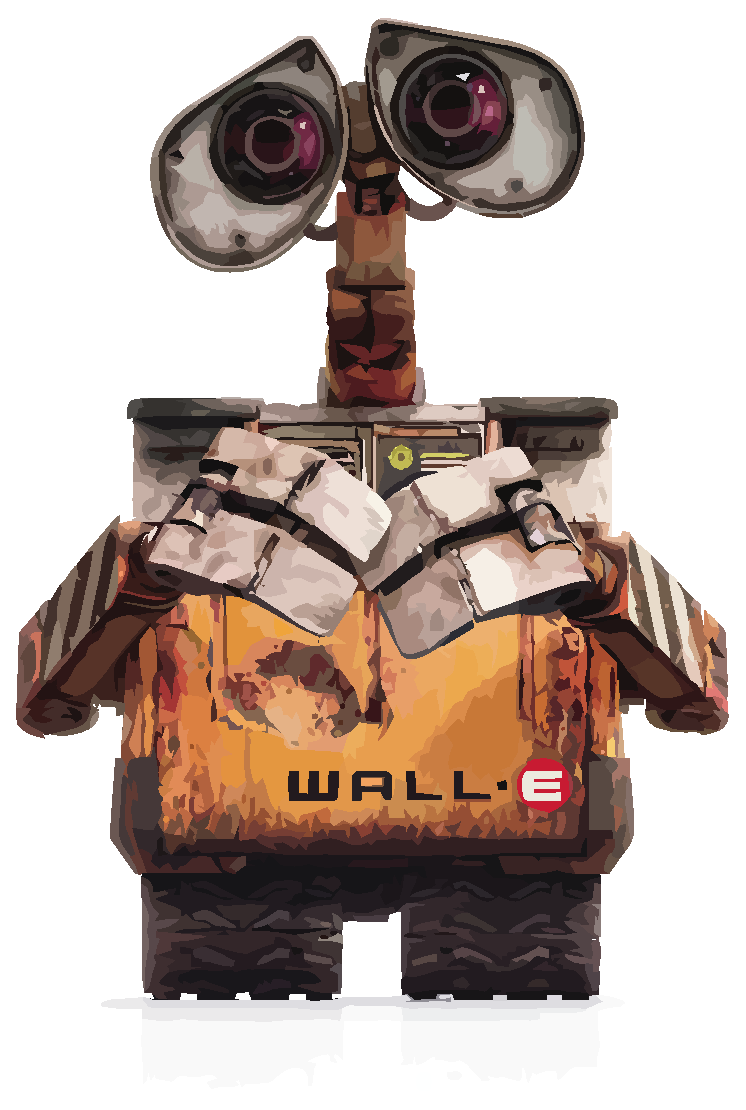
\includegraphics[width=\textwidth]{WallE}
    \caption{Wall-E}
    \label{fig:WallE}
  \end{subfigure}             
  \begin{subfigure}[b]{0.3\textwidth}
    
\includegraphics[width=\textwidth]{minion}
    \caption{Minions}
    \label{fig:Minnion}
  \end{subfigure}
  \caption{Best Animations}
  \label{fig:animations}
\end{figure}


\end{landscape}

%%!TEX root = ../thesis.tex
%*******************************************************************************
%****************************** Third Chapter **********************************
%*******************************************************************************
\chapter{My third chapter}

% **************************** Define Graphics Path **************************
\ifpdf
    \graphicspath{{Chapter3/Figs/Raster/}{Chapter3/Figs/PDF/}{Chapter3/Figs/}}
\else
    \graphicspath{{Chapter3/Figs/Vector/}{Chapter3/Figs/}}
\fi

\section{First section of the third chapter}
And now I begin my third chapter here \dots

And now to cite some more people~\citet{Rea85,Ancey1996}

\subsection{First subsection in the first section}
\dots and some more 

\subsection{Second subsection in the first section}
\dots and some more \dots

\subsubsection{First subsub section in the second subsection}
\dots and some more in the first subsub section otherwise it all looks the same
doesn't it? well we can add some text to it \dots

\subsection{Third subsection in the first section}
\dots and some more \dots

\subsubsection{First subsub section in the third subsection}
\dots and some more in the first subsub section otherwise it all looks the same
doesn't it? well we can add some text to it and some more and some more and
some more and some more and some more and some more and some more \dots

\subsubsection{Second subsub section in the third subsection}
\dots and some more in the first subsub section otherwise it all looks the same
doesn't it? well we can add some text to it \dots

\section{Second section of the third chapter}
and here I write more \dots

\section{The layout of formal tables}
This section has been modified from ``Publication quality tables in \LaTeX*''
 by Simon Fear.

The layout of a table has been established over centuries of experience and 
should only be altered in extraordinary circumstances. 

When formatting a table, remember two simple guidelines at all times:

\begin{enumerate}
  \item Never, ever use vertical rules (lines).
  \item Never use double rules.
\end{enumerate}

These guidelines may seem extreme but I have
never found a good argument in favour of breaking them. For
example, if you feel that the information in the left half of
a table is so different from that on the right that it needs
to be separated by a vertical line, then you should use two
tables instead. Not everyone follows the second guideline:

There are three further guidelines worth mentioning here as they
are generally not known outside the circle of professional
typesetters and subeditors:

\begin{enumerate}\setcounter{enumi}{2}
  \item Put the units in the column heading (not in the body of
          the table).
  \item Always precede a decimal point by a digit; thus 0.1
      {\em not} just .1.
  \item Do not use `ditto' signs or any other such convention to
      repeat a previous value. In many circumstances a blank
      will serve just as well. If it won't, then repeat the value.
\end{enumerate}

A frequently seen mistake is to use `\textbackslash begin\{center\}' \dots `\textbackslash end\{center\}' inside a figure or table environment. This center environment can cause additional vertical space. If you want to avoid that just use `\textbackslash centering'


\begin{table}
\caption{A badly formatted table}
\centering
\label{table:bad_table}
\begin{tabular}{|l|c|c|c|c|}
\hline 
& \multicolumn{2}{c}{Species I} & \multicolumn{2}{c|}{Species II} \\ 
\hline
Dental measurement  & mean & SD  & mean & SD  \\ \hline 
\hline
I1MD & 6.23 & 0.91 & 5.2  & 0.7  \\
\hline 
I1LL & 7.48 & 0.56 & 8.7  & 0.71 \\
\hline 
I2MD & 3.99 & 0.63 & 4.22 & 0.54 \\
\hline 
I2LL & 6.81 & 0.02 & 6.66 & 0.01 \\
\hline 
CMD & 13.47 & 0.09 & 10.55 & 0.05 \\
\hline 
CBL & 11.88 & 0.05 & 13.11 & 0.04\\ 
\hline 
\end{tabular}
\end{table}

\begin{table}
\caption{A nice looking table}
\centering
\label{table:nice_table}
\begin{tabular}{l c c c c}
\hline 
\multirow{2}{*}{Dental measurement} & \multicolumn{2}{c}{Species I} & \multicolumn{2}{c}{Species II} \\ 
\cline{2-5}
  & mean & SD  & mean & SD  \\ 
\hline
I1MD & 6.23 & 0.91 & 5.2  & 0.7  \\

I1LL & 7.48 & 0.56 & 8.7  & 0.71 \\

I2MD & 3.99 & 0.63 & 4.22 & 0.54 \\

I2LL & 6.81 & 0.02 & 6.66 & 0.01 \\

CMD & 13.47 & 0.09 & 10.55 & 0.05 \\

CBL & 11.88 & 0.05 & 13.11 & 0.04\\ 
\hline 
\end{tabular}
\end{table}


\begin{table}
\caption{Even better looking table using booktabs}
\centering
\label{table:good_table}
\begin{tabular}{l c c c c}
\toprule
\multirow{2}{*}{Dental measurement} & \multicolumn{2}{c}{Species I} & \multicolumn{2}{c}{Species II} \\ 
\cmidrule{2-5}
  & mean & SD  & mean & SD  \\ 
\midrule
I1MD & 6.23 & 0.91 & 5.2  & 0.7  \\

I1LL & 7.48 & 0.56 & 8.7  & 0.71 \\

I2MD & 3.99 & 0.63 & 4.22 & 0.54 \\

I2LL & 6.81 & 0.02 & 6.66 & 0.01 \\

CMD & 13.47 & 0.09 & 10.55 & 0.05 \\

CBL & 11.88 & 0.05 & 13.11 & 0.04\\ 
\bottomrule
\end{tabular}
\end{table}

%\include{Chapter4/chapter4}
%\include{Chapter5/chapter5}
%\include{Chapter6/chapter6}
%\include{Chapter7/chapter7}



% ********************************** Back Matter *******************************
% Backmatter should be commented out, if you are using appendices after References
%\backmatter

% ********************************** Bibliography ******************************
\begin{spacing}{0.9}

% To use the conventional natbib style referencing
% Bibliography style previews: http://nodonn.tipido.net/bibstyle.php
% Reference styles: http://sites.stat.psu.edu/~surajit/present/bib.htm

%\bibliographystyle{apalike}
\bibliographystyle{unsrtnat} % Use for unsorted references  
%\bibliographystyle{plainnat} % use this to have URLs listed in References
\cleardoublepage
\bibliography{References/references} % Path to your References.bib file


% If you would like to use BibLaTeX for your references, pass `custombib' as
% an option in the document class. The location of 'reference.bib' should be
% specified in the preamble.tex file in the custombib section.
% Comment out the lines related to natbib above and uncomment the following line.

%\printbibliography[heading=bibintoc, title={References}]


\end{spacing}

% ********************************** Appendices ********************************

\begin{appendices} % Using appendices environment for more functunality

\chapter{Risk Assessment Retrospective}
In risk assessment submitted it October, it was noted that the risks related to this project would be due to extensive computer usage. This risk assessment proved to be accurate and the appropriate steps were taken to mitigate these risks, including ensuring appropriate working conditions, suitable posture and a sensible working pattern. 

\chapter{Electronic Resources}
Please note that all code listings for this project may be found on \texttt{GitHub} at this address: \url{https://github.com/MrinankSharma/dp-pvi-project}. 

Additionally, the electronic log book used for this project can be found at the following address: \url{https://drive.google.com/file/d/1PafemIYA0pPCeIDv2K_utI8CYklXyPmM/view?usp=sharing}.
%%!TEX root = ../thesis.tex
% ******************************* Thesis Appendix B ********************************

\chapter{Installing the CUED class file}

\LaTeX.cls files can be accessed system-wide when they are placed in the
<texmf>/tex/latex directory, where <texmf> is the root directory of the user’s \TeX installation. On systems that have a local texmf tree (<texmflocal>), which
may be named ``texmf-local'' or ``localtexmf'', it may be advisable to install packages in <texmflocal>, rather than <texmf> as the contents of the former, unlike that of the latter, are preserved after the \LaTeX system is reinstalled and/or upgraded.

It is recommended that the user create a subdirectory <texmf>/tex/latex/CUED for all CUED related \LaTeX class and package files. On some \LaTeX systems, the directory look-up tables will need to be refreshed after making additions or deletions to the system files. For \TeX Live systems this is accomplished via executing ``texhash'' as root. MIK\TeX users can run ``initexmf -u'' to accomplish the same thing.

Users not willing or able to install the files system-wide can install them in their personal directories, but will then have to provide the path (full or relative) in addition to the filename when referring to them in \LaTeX.

\end{appendices}

% *************************************** Index ********************************
\printthesisindex % If index is present

\end{document}
